\chapter{Validation of Application Energy Monitoring}
\label{chapter:validation}

\section{Introduction}

As described in \cref{chapter:implementation} we have implemented a proof-of-concept version of the Apollo Energy Allocator system, to prove the usefulness of our approach for allocating energy of underlying host systems to individual application requests running on them.  The software was tested during development to ensure correctness with respect to expected results through unit and integration tests, but now needs to be validated by using it in realistic test cases.  This process is described in this chapter.

In order to validate Apollo with realistic test cases, we need to define the kind of validation we are interested in achieving.  There are two main varieties of validation that we wish to achieve.

Firstly we wish to validate the \emph{consistency} of Apollo's results across a range of scenarios, to ensure that energy is allocated consistently with respect to the workload in the execution scenarios and host utilisation levels that prevail during them.

Next, we need to validate the \emph{allocation} of Apollo's results when a specific application scenario is run on a host machine with different amounts of competing workload.  As the competing workload rises, the energy allocation to the application scenario should fall, in proportion to its use of the machine.

We also wish to validate the \emph{calculation correctness} of Apollo's results, by running the calculator in one or more controlled scenarios where we can also gather additional runtime statistics that allow a separate independent calculation of a fair energy consumption and manually perform these calculations and use them to check the correctness of Apollo's results in the same scenarios.

Finally, an additional area of validation we wish to perform is to confirm that \emph{CPU is a valid proxy for overall resource usage} when performing energy allocation calculations.  For this validation we focus on how CPU usage varies for disk IO intensive workloads.

\section{Testing Approach}

\subsection{The Test Application}
TODO - explain the microservice app

\subsection{The Test Software}
TODO - explain how tests were run and results captured including machine type, scripting, data capture and synthetic workload.

\section{Validating Consistency}

To validate consistency of energy allocation, our strategy is to run a known control workload under fixed host utilisation conditions (no other workload being the simplest case) and to run a range of other workloads that we know contain an equivalent amount of computational work but are structured differently.  The energy allocation should be the same for each case.

In our first test, we structured a workload into three cases, each of which involved the same amount of CPU workload but in three different scenarios.  The first scenario invoked a short service call (involving 50msec of CPU work) 1000 times, the second scenario invoked a longer service call (500msec of CPU work) 100 times and the third ran a long service call (5000msec of CPU work) 10 times.  Each scenario was called 6 times to ensure a consistent result.

Our first question was whether the energy allocations per request were consistent across the three cases.  Our analysis of this question is shown in the scatter graph in \fref{figure:validation-energycpu}, which plots the energy usage against CPU workload for each of the scenarios executed, using logarithmic scales.

\begin{figure}
\centering
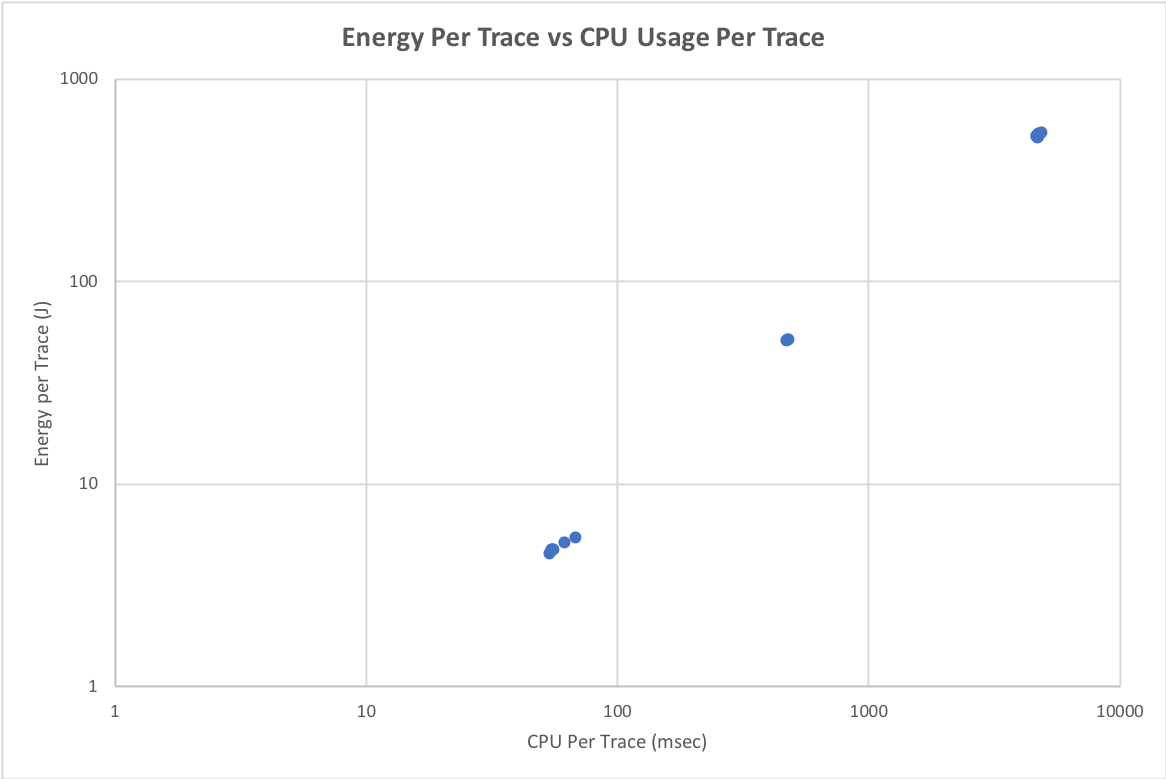
\includegraphics[width=1.0\textwidth]{Figures/validation-energycpu}
\caption{Energy Allocation per Request for Small, Medium and Large Services}
\label{figure:validation-energycpu}
\end{figure}

The graph shows the three sets of scenarios (short, medium and long) clearly clustering very closely, showing that the energy allocation per trace is extremely consistent across the three sets, suggesting that the allocation calculation is working consistently as designed.  More precisely, the correlation coeficient between the two sets of values is 0.999, indicating a very high degree of correlation between CPU consumed and energy allocation performed.

We also wanted to understand how consistent the energy allocation per trace was across the three service request sets and to do this we calculated the CPU to energy ratio as $CPU msec / Energy J$ for each of the results we had from this test set.  The results of this calculation are presented in \tref{table:energypermsec}.

\begin{table}
\centering
\caption{Energy Allocation per Millisecond}
\label{table:energypermsec}
\footnotesize
\begin{tabular}{|l|r|r|}
\hline
\textbf{Request Length} & \textbf{Average J/msec}  & \textbf{Stddev J/msec} \\
\hline
50 msec & 0.0848 & 0.0026 \\
\hline
500 msec & 0.1094 & 0.0005 \\
\hline
5000 msec & 0.1121 & 0.0017 \\
\hline
\end{tabular}
\end{table} 

As can be seen, the energy allocation per CPU millisecond is slightly different between the three cases, with a consistent trend to increase slightly as the number of milliseconds of CPU time per request increases by an order of magnitude each time.  As can also be seen the standard deviation values are very small, indicating that the averages are representative of the data.

When we analysed these values a little we noticed that the difference between the average for the 50 msec case and the 500 msec case was 0.0246, while the difference between the 500 msec case and the 5000 msec case was 0.0027.  So the difference in mean values differs by the same order of magnitude as the length of the workload in each case.  The length of the workload is inversely proportional to the number of service requests made, therefore we think the lower energy per millisecond for the short requests indicates the lower intensity of workload that the scenario places the server under.  As much of the time in this scenario will be waiting for network operations to receive or transmit data from and to the client, the intensity of the CPU operation will be lower and so the allocation algorithm results in a (slightly) lower amount of energy per CPU millisecond of work. [\textbf{TODO} - really?  Need to think this out in detail.]

Our second test involved investigating how energy allocation was affected by a constant amount of CPU workload but in scenarios of different lengths.  To test this we ran repeatedly ran two scenarios, both of which contained the same amount of CPU workload (a trace that took 2,500 msec, run 50 times), with one scenario having pauses inserted into it, to cause the scenario to take longer to execute but consume no more CPU resource during the extended execution time.  In addition, for reasons which we explain below, we ran the first set of scenario tests with no additional load on the machine and the second set with synthetic workload consuming 50\% of the machine's CPU.  The results of this experiment are shown in the line graph in \fref{figure:validation-scenariolength}

\begin{figure}
\centering
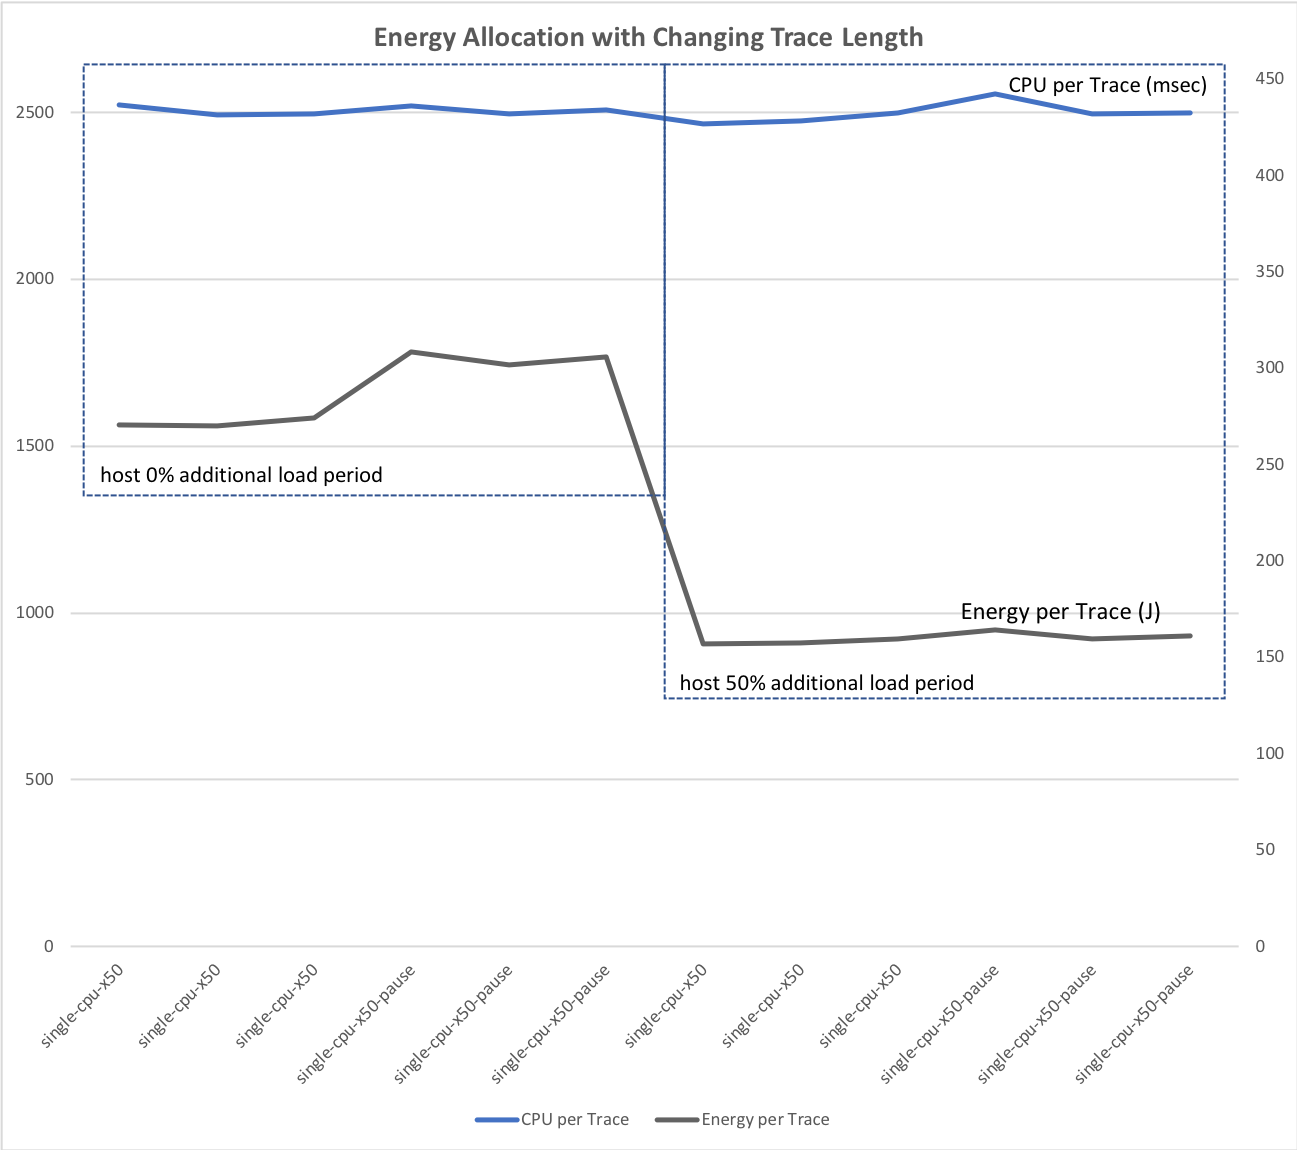
\includegraphics[width=1.0\textwidth]{Figures/validation-scenariolength}
\caption{Energy Allocation Across Different Scenario Lengths}
\label{figure:validation-scenariolength}
\end{figure}

This graph plots the CPU usage per trace (the top line) and the energy usage per trace (the bottom line) for sample executions of the scenarios.  As indicated by the dashed boxes annotating the graph, the first 6 executions were performed with no additional workload on the machine, the second 6 executions were performed with the machine having 50\% of its CPU capacity consumed by other synthetic workload.

As can be seen from the graph, the estimate of CPU usage by trace is consistent, within a maximum of 2\% variation from the mean (min 2467, max 2556, mean 2502, std deviation of 23.09, which is less than 1\% of the mean).  This is well within our target consistency.

When we analysed the power allocation by trace we saw an interesting development which was the higher power allocation for the longer scenarios when no additional load was on the machine, an in constrast, a more constant power allocation when 50\% additional load was running on the machine.  While unintuitive initially, this is exactly as expected and is an important energy usage insight for the software architect investigating the power characteristics of their software in production.  

When no additional load is executing on the host, there is no other workload apart from our traces to allocate power consumption to.  In which case if the scenario takes longer, you would expect a higher energy allocation even with constant resource usage, as the host machine is consuming energy, even when not actively running our workload and if there is no other workload to allocate this "background" energy consumption to, then it will be allocated to our workload.  The graph shows that this is exactly what happens; when no other workload is executing on the machine, our longer scenarios (the "single-cpu-x50-pause" scenarios) are allocated more power than the shorter scenarios (the "single-cpu-x50" ones) even though they all consume very similar amounts of CPU time.

In contrast, when there is additional workload on the machine, the energy allocated to each trace is much more even, within a maximum of 4\% variation from the mean (min 157, max 164, mean 160, std deviation of 2.66 which is 1.6\% of the mean).  This is also an expected result as during the execution of our test workload, there is other workload running on the machine which shares the allocation of the host's energy consumption.  As our workload runs longer, but is not using CPU during part of the period, it is allocated correspondingly less of the host's energy as there is other active workload on the machine which is allocated more of it.  This is the alocation we would expect and it is within our target consistency and again suggests that this is a consistent energy allocation mechanism.

\section{Validating Allocation}

Another aspect of energy allocation is how a fixed workload is allocated energy when the underlying host has varying amounts of other workload running on it concurrently.  We tested this aspect of allocation by running a single workload type under 5 different host utilisation conditions, namely when there was no other workload on the host, and when the host was 25\%, 50\%, 75\% and 100\% utilised before our workload started.  The results of this test are shown in the line graph in \fref{figure:validation-machineload}.

\begin{figure}
\centering
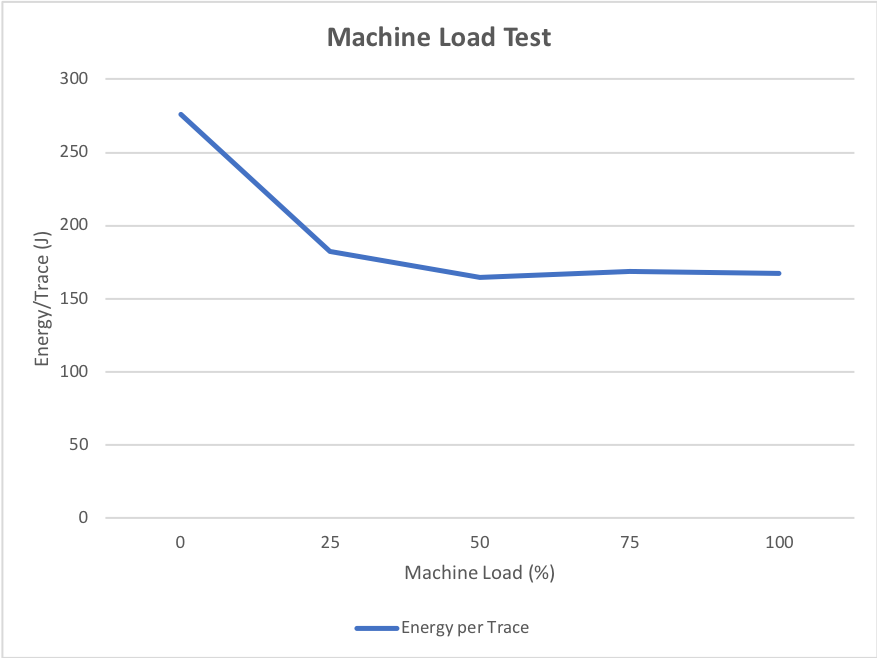
\includegraphics[width=1.0\textwidth]{Figures/validation-machineload}
\caption{Energy Allocation Under Different Host Load Conditions}
\label{figure:validation-machineload}
\end{figure}

As with some of our other testing, the results initially look somewhat counter intuitive, but on further analysis are validation of consistent energy allocation by workload.

%  (Trace J at 25/50/75/100 prior load: 276, 183 [93], 164 [19], 169, 167)

The first point in the graph shows our workload running on an otherwise idle host and it is allocated quite a large amount of energy per trace (of 276J) because the host is relatively inefficient at lower levels of utilisation and there is no other workload on the host to allocate its energy to.

The second point in the graph shows a sharp reduction in energy per trace (to 183J), which is caused by the host's utilisation now being about 50\% which is considerably more efficient than 25\% and the fact that the host's energy is being split between two roughly equivalent workloads.

The third point on the graph shows a further reduction in energy per trace (to 164J), which is a considerably smaller reduction than the previous step.  This is due to our share of the machine workload falling less significantly than in the previous step (from 49\% to 33\% whereas the previous step was from 96\% to 49\%).

The fourth point on the graph, at 75\% of other utilisation, actually goes up slightly (to 169J).  This is due to two factors.  Firstly, once again, our utilisation percentage drop decreases, this time from 33\% to 25\% (only 8\%) but secondly, the underlying machine becomes less efficient as utilisation moves beyond 75\% and so there is more energy to allocate between the different workload items.  This is an important insight for the application architect so that they consider the potentially non-linear energy consumption curve of the underlying host.

Finally at the fifth point on the graph, with 100\% other utilisation, our workload is competing with existing workload to be scheduled for execution.  This results in our execution duration extending slightly (by 5\%), and our CPU utilisation percentage to drop slightly (to 23\%) with the result being a slight reduction in energy utilisation (to 167J).  This is the result of a relatively small increase in the host's energy utilisation (as it was already running close to 100\% utilisation at the previous sample) and there is now further workload to allocate the energy of the host across, so reducing our workload's allocation slightly.

This testing was interesting to us because it showed the usefulness of investigating energy allocation using practical testing and a quantitative data-based allocation mechanism like Apollo.  It would be quite possible to make a simplistic assumption that fair energy allocation would keep falling linearly as load increased, but our tool can be used to provide a more sophisticated analysis that reveals how a complex interaction of a number of factors (including load, scenario length and host energy characteristics) can result in a correct allocation that is more complex.  This is a useful insight for the application architect as they investigate the energy characteristics of their application.

\section{Validating Calculation}

\section{Validating CPU as a Resource Usage Proxy}

\section{Summary}

